\documentclass [border = .2cm] {standalone}

% Required packages
\usepackage{pgfplots}
\pgfplotsset{compat = newest}
\usetikzlibrary {backgrounds}

\begin{document}
	
	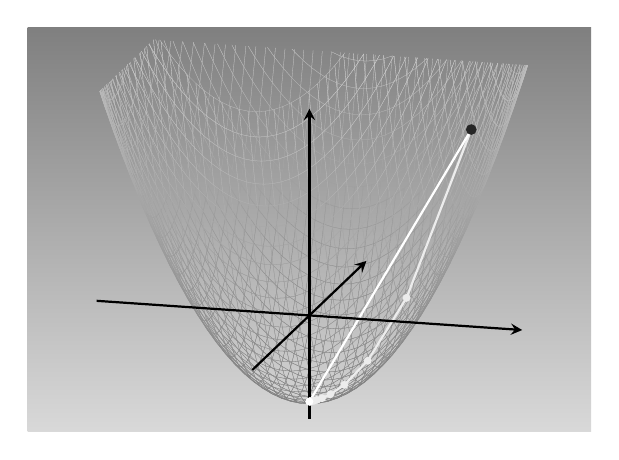
\begin{tikzpicture}		
		[background rectangle/.style=
		{bottom color=white!70!gray!},
		show background rectangle]
		
		\begin{axis}[
			 view = {15}{20},
			 colormap={blackwhite}{gray(0cm)=(0.5); gray(1cm)=(1)},
			 thick,
			 axis lines = center,
			 axis on top,
			 color=black,
			 xmax = 10,
			 xmin = -10,
			 ymax = 10, 
			 ymin = -10, 
			 zmax = 12, 
			 zmin = -6,
			 xticklabels=\empty,
			 yticklabels=\empty,
			 zticklabels=\empty,
			 xtick=false,
			 ytick=false,
			 ztick=false,
			 ]
			
			\addplot3 [
			domain=-10:10,
			domain y = -10:10,
			samples = 50,
			samples y = 50,
			surf,
			mesh,
			ultra thin,
			shader = interp,
			no marks,
			] {0.2 * x^2 + 0.2 * y^2 - 5};
			
					
			\addplot3 [
			color=white!85!gray!,
			thick,
			mark=*,	
			mark size=1pt,		
			draw=white!85!gray!,
			] coordinates 
			{
				(6, 6, 9.4)
				(3.60000000000000, 3.60000000000000, 0.183999999999999)	
				(2.16000000000000, 2.16000000000000, -3.13376000000000)
				(1.29600000000000, 1.29600000000000, -4.32815360000000)
				(0.777600000000001, 0.777600000000001, -4.75813529600001)
				(0.466560000000000, 0.466560000000000, -4.91292870656001)
				(0.279936000000000, 0.279936000000000, -4.96865433436160)
				(0.167961600000000, 0.167961600000000, -4.98871556037018)
				(0.100776960000000, 0.100776960000000, -4.99593760173327)
				(0.0604661760000000, 0.0604661760000000, -4.99853753662398)
				(0.0362797056000000, 0.0362797056000000, -4.99947351318464)
				(0.0217678233600000, 0.0217678233600000, -4.99981046474647)
				(0.0130606940160000, 0.0130606940160000, -4.99993176730873)
				(0.00783641640960000, 0.00783641640960000, -4.99997543623115)
				(0.00470184984576000, 0.00470184984576000, -4.99999115704322)
			};
		
		    \addplot3 [
		    color=white,
		    thick,
		    mark=*,
		    mark size=1pt,
		    draw=white,			
		    ] coordinates 
		    {
		    	(6, 6, 9.4)
		    	(0,0,-5)
		    };
		    
			\addplot3 [
			color=gray!30!black!,
			mark=*,	
			mark size=1.5pt,	
			] coordinates 
			{
				(6, 6, 9.4)
				
			};
			
				
		\end{axis}
		
	\end{tikzpicture}
	
\end{document}